\documentclass[12pt,svgnames,]{beamer}
\usepackage{etex} % Uncomment if shortage of latex registers
\usepackage[utf8]{inputenc}
\usepackage[T1]{fontenc}
\usepackage[english]{babel}
\usepackage{enumerate}
\usepackage{lmodern}
\setbeamertemplate{navigation symbols}{}
\usepackage{graphicx}
\usepackage{amsmath}
\usepackage{caption}
\usetheme{/amsterdam}
\date{23. Juni 2015}
\usepackage{listings}
\lstset{literate=%
{Ø}{{\O}}1
{Å}{{\AA}}2
{Æ}{{\AE}}2
{ø}{{\o}}1
{å}{{\aa}}2
{æ}{{\ae}}2
}
\graphicspath{{pictures/}}

\begin{document}
\captionsetup[figure]{font=small,singlelinecheck=off,justification=raggedright}
\title[Bachelor Project exam sw605f15]{GIRAF}
\author[slide \insertframenumber /\inserttotalframenumber]{sw605f15, Aalborg University}
\frame{\maketitle\thispagestyle{empty}}

\begin{frame}
  \frametitle{Contents}
  \tableofcontents
\end{frame}

\section{GIRAF}
\begin{frame}
	\frametitle{GIRAF Project}
\end{frame}

\subsection{GIRAF Overview}

\begin{frame}
  \begin{center}
	\frametitle{Multiproject}
  \end{center}
\end{frame}

\begin{frame}
	\begin{center}
		\frametitle{Goals for the semester}
		\begin{itemize}
			\item \textit{A product that actually works and can be used} - 10/02-15
			\item Build upon existing features
			\item Quality over quantity
		\end{itemize}
	\end{center}
\end{frame}

\begin{frame}
	\frametitle{Roles and responsibility}
	\begin{columns}[T] % align columns
		\begin{column}{.48\textwidth}
			\begin{itemize}
				\item Redmine Wiki, Forum, general
				\item Server
				\item Webadmin
				\item Graphics/Fonts/etc
				\item Customer Representatives
				\item Git Handling
			\end{itemize}
		\end{column}%
		\hfill%
		\begin{column}{.48\textwidth}
			\begin{itemize}
				\item 
				\item code style
				\item Jenkins
				\item Scrum Process
				\item \textbf{Google Play}
				\item \textbf{Google Analytics}
				\item \textbf{Product Owners}
			\end{itemize}
		\end{column}%
	\end{columns}
\end{frame}

\begin{frame}
	\begin{center}
		\frametitle{Project Struture}
		\begin{columns} % align columns
			\begin{column}{.3\textwidth}
				Scrum of Scrums
				\begin{itemize}
					\item 1 Scrum Lord
					\item 3 Subprojects
					\item 15 groups
					\item 48 students
				\end{itemize}
			\end{column}%
			\begin{column}{.80\textwidth}
				\begin{figure}[H]
					\centering
					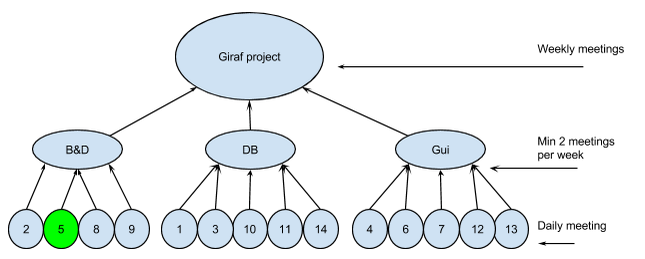
\includegraphics[width= 0.8 \textwidth]{pictures/ScrumOfScrum.png}
				\end{figure}
			\end{column}%
		\end{columns}
	\end{center}
\end{frame}

\begin{frame}
	\begin{center}
		\frametitle{Redmine}
		\begin{figure}[H]
			\centering
			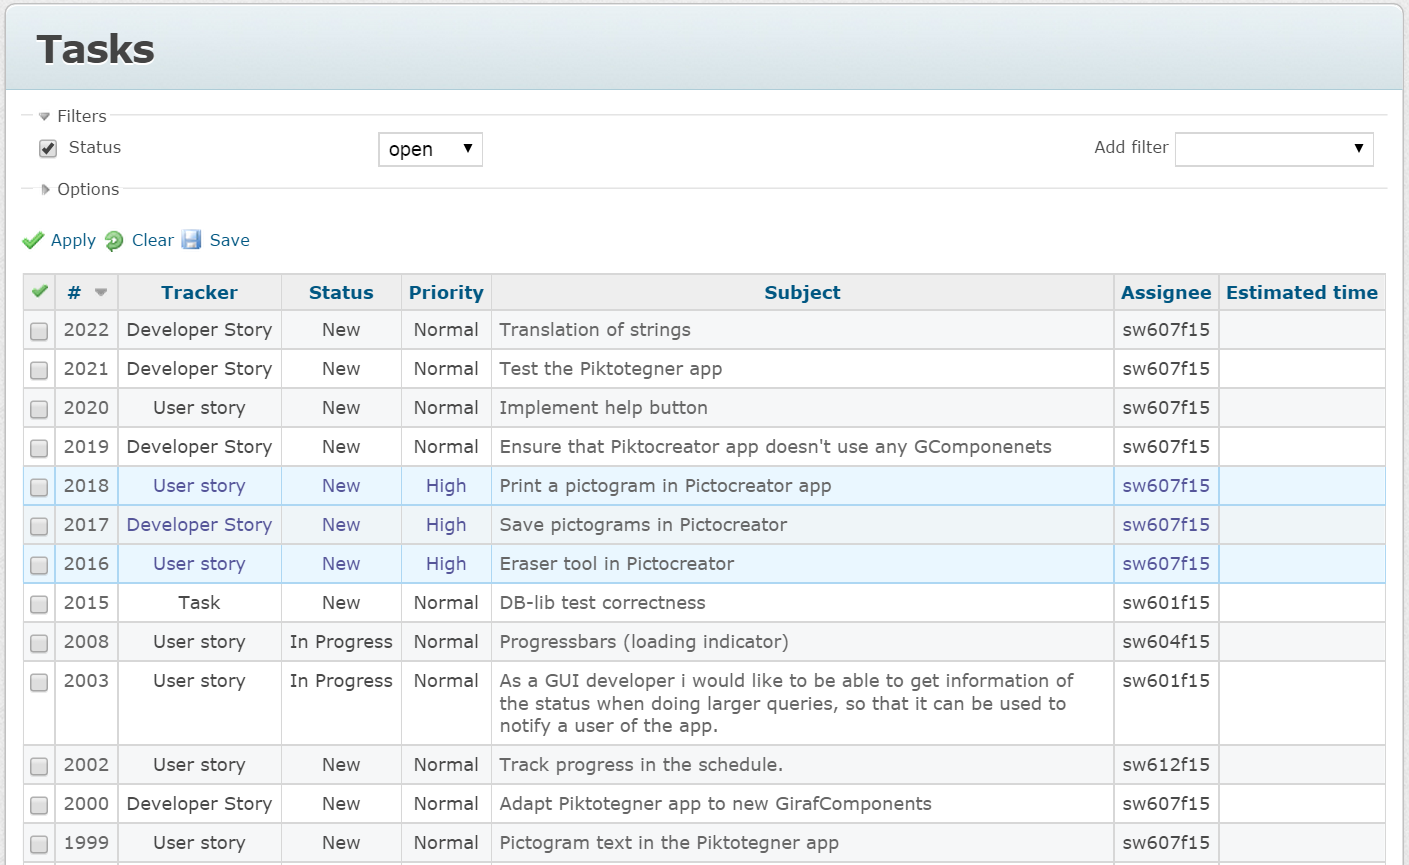
\includegraphics[width= 0.8 \textwidth]{pictures/RedmineStory.png}
		\end{figure}
	\end{center}
\end{frame}

\section{Product Owner}

\begin{frame}
	\begin{center}
		\frametitle{Responsibilities}
		\begin{columns}[T] % align columns
			\begin{column}{.48\textwidth}
				\begin{itemize}
					\item User stories
						\begin{itemize}
							\item Product Backlog
							\item Release Backlog
						\end{itemize}
					\item Sprint Planning
					\item Sprint End
					\item Communicate with other PO-groups
				\end{itemize}
			\end{column}%
			\hfill%
			\begin{column}{.48\textwidth}
				\begin{figure}[H]
					\centering
					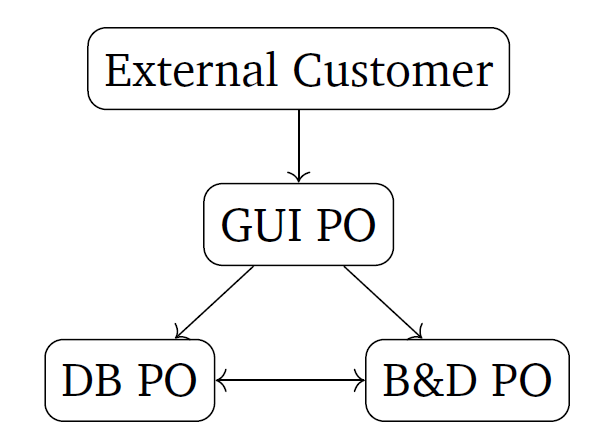
\includegraphics[width= 0.8 \textwidth]{pictures/ProductOwnerRelation.png}
				\end{figure}
			\end{column}%
		\end{columns}
	\end{center}
\end{frame}

\subsection{User stories}

\begin{frame}
	\begin{center}
		\frametitle{User stories}
	\end{center}
\end{frame}

\subsection{Backlog}

\begin{frame}
	\begin{center}
		\frametitle{Product Backlog}
	\end{center}
\end{frame}

\begin{frame}
	\begin{center}
		\frametitle{Release Backlog}
	\end{center}
\end{frame}
			%Introduction + PO by Lukas
\section{Google Play and Analytics}
\subsection{Google Play}
\begin{frame}
	\frametitle{Google Play}
	\begin{figure}[H]
		\centering
		
\includegraphics[width= 0.8 \textwidth]{pictures/Play_icon.jpg}
	\end{figure}
\end{frame}

\begin{frame}
	\begin{center}
		\frametitle{Releasing the apps}
		\begin{columns}[T] % align columns
			\begin{column}{.3\textwidth}
				1st and 2nd sprint
				\begin{itemize}
					\item Manual releases
					\item Was troublesome
				\end{itemize}
			\end{column}%
			\begin{column}{.3\textwidth}
				3rd and 4th sprint
				\begin{itemize}
					\item Automated upload
					\item Versions always tested
				\end{itemize}
			\end{column}%
	\end{columns}
	\end{center}
\end{frame}

\begin{frame}
	\begin{center}
		\frametitle{Release versions}
		\begin{columns} % align columns
			\begin{column}{.3\textwidth}
				Versions on Google Play
				\begin{itemize}
					\item Access to versions
				\end{itemize}
			\end{column}%
			\begin{column}{.80\textwidth}
				\begin{figure}[H]
					\centering
					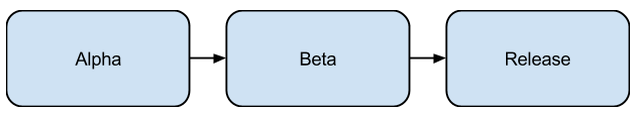
\includegraphics[width= 0.8 \textwidth]{pictures/Versions.png}
				\end{figure}
			\end{column}%
		\end{columns}
	\end{center}
\end{frame}

\begin{frame}
	\begin{center}
		\frametitle{Testing access}
		\begin{columns} % align columns
			\begin{column}{.3\textwidth}
				Who have access to what
			\end{column}%
			\begin{column}{.80\textwidth}
				\begin{figure}[H]
					\centering
					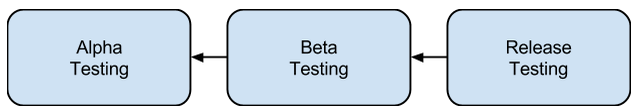
\includegraphics[width= 0.8 \textwidth]{pictures/Access.png}
				\end{figure}
			\end{column}%
		\end{columns}
	\end{center}
\end{frame}

\subsection{Google Analytics}
\begin{frame}
	\frametitle{Google Analytics}
	\begin{figure}[H]
		\centering
		
\includegraphics[width= 0.5 \textwidth]{pictures/analytics_icon.png}
	\end{figure}
\end{frame}

\begin{frame}
	\begin{center}
		\frametitle{Google Analytics}
		\begin{columns}[T] % align columns
			\begin{column}{.3\textwidth}
				What it does
				\begin{itemize}
					\item Crash reports
					\item Statistics
				\end{itemize}
			\end{column}%
			\begin{column}{.3\textwidth}
				How we used it
				\begin{itemize}
					\item Transitioned away from it 
					\item Jenkins helped
				\end{itemize}
			\end{column}%
		\end{columns}
	\end{center}
\end{frame}

\subsection{Renaming}
\begin{frame}
	\frametitle{Renaming of Package-names}
	\begin{figure}[H]
		\centering
		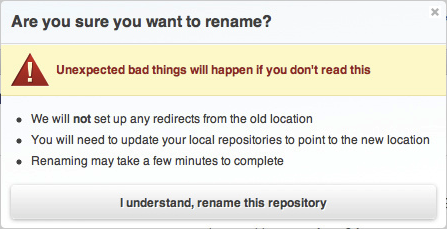
\includegraphics[width= 0.8 \textwidth]{pictures/Renaming.png}
	\end{figure}
\end{frame}

\begin{frame}
	\begin{center}
		\frametitle{Renaming process}
		\begin{columns} % align columns
			\begin{column}{.9\textwidth}
				\begin{tabular}{ll}
					\textbf{Old app package-names} & \textbf{New app package-names}\\ \hline \noalign{\vskip 2mm}
					launcher & launcher\\ \hline
					train & categorygame\\ \hline
					pictoadmin & categorymanager\\ \hline
					tortoise & lifestory\\ \hline
					oasis & administration\\ \hline
					parrot & pictoreader\\ \hline
					pictosearch & pictosearch\\ \hline
					pictocreator & pictocreator\\ \hline
					zebra & sequence\\ \hline
					cars & voicegame\\ \hline
					wombat & timer\\ \hline
					schedulestarter & ugeplan\\ \hline
				\end{tabular}
			\end{column}%
		\end{columns}
	\end{center}
\end{frame}			%Google Play and Google Analytics by Claus
\input{contents/Build Structure}			%How we changed the build structure by Martin
\section{StandAlone}
\begin{frame}
	\frametitle{App dependencies}
	
\end{frame}
\begin{frame}
	\frametitle{Solution Ideers}

\end{frame}
\begin{frame}
	\frametitle{Problems}

\end{frame}				%Standalone by Martin 
\subsection{Package solution}
\begin{frame}
	\frametitle{Package solution}
\end{frame}

\begin{frame}
	\begin{center}
		\frametitle{Download one place}
		\begin{figure}[H]
			\centering
			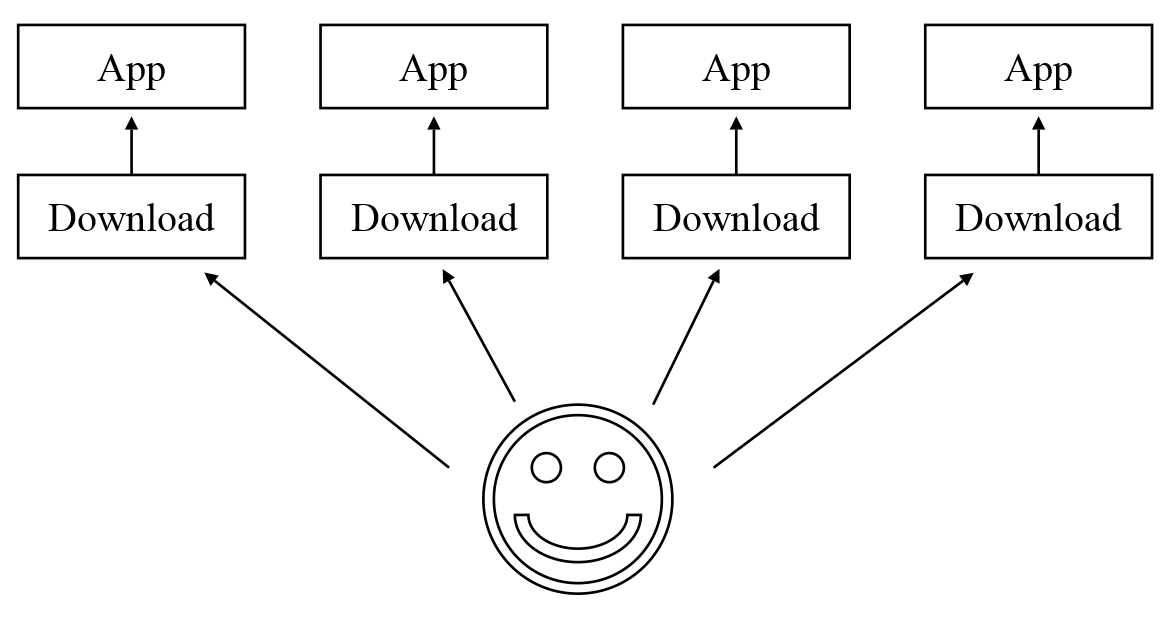
\includegraphics[width= 0.8 \textwidth]{pictures/MultipleDownload.png}
		\end{figure}
	\end{center}
\end{frame}

\begin{frame}
	\begin{center}
		\frametitle{Download one place}
		\begin{figure}[H]
			\centering
			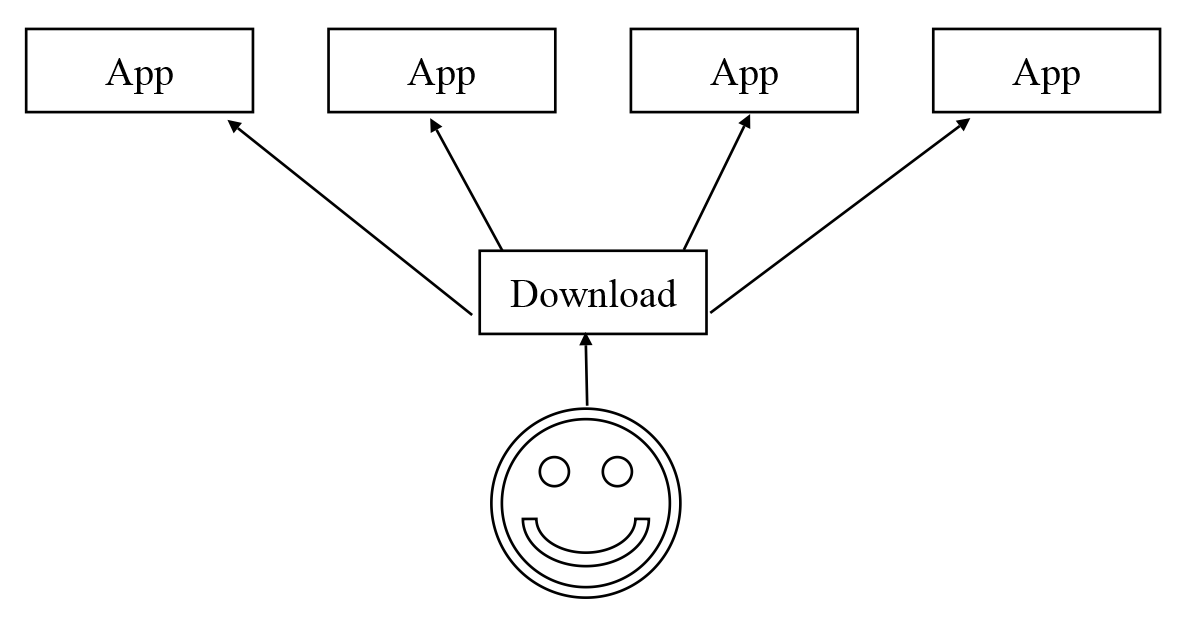
\includegraphics[width= 0.8 \textwidth]{pictures/DownloadOnePlace.png}
		\end{figure}
	\end{center}
\end{frame}

\begin{frame}
	\begin{center}
		\frametitle{Make one app}
		\begin{figure}[H]
			\centering
			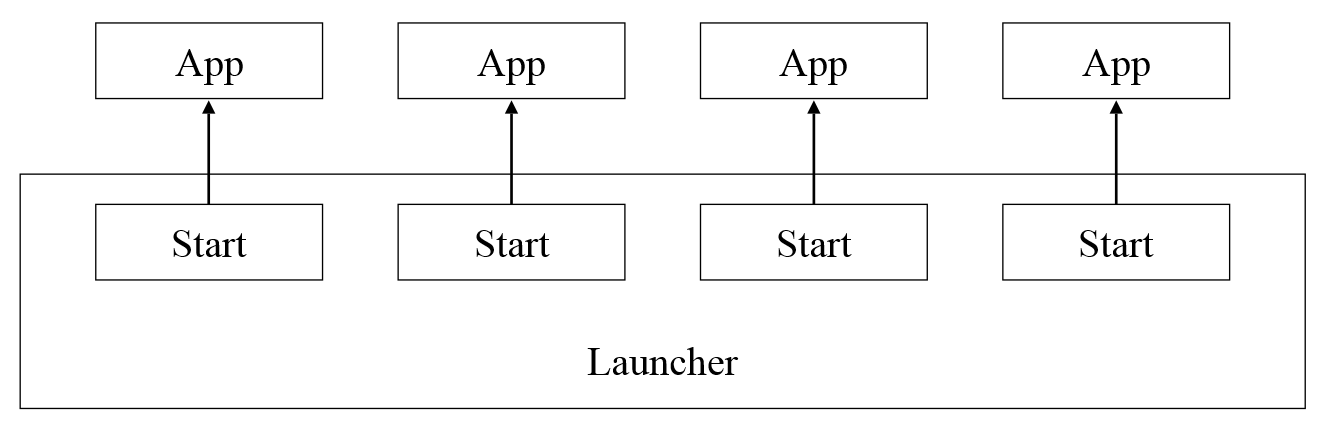
\includegraphics[width= 0.8 \textwidth]{pictures/OldLauncher.png}
		\end{figure}
	\end{center}
\end{frame}

\begin{frame}
	\begin{center}
		\frametitle{Make one app}
		\begin{figure}[H]
			\centering
			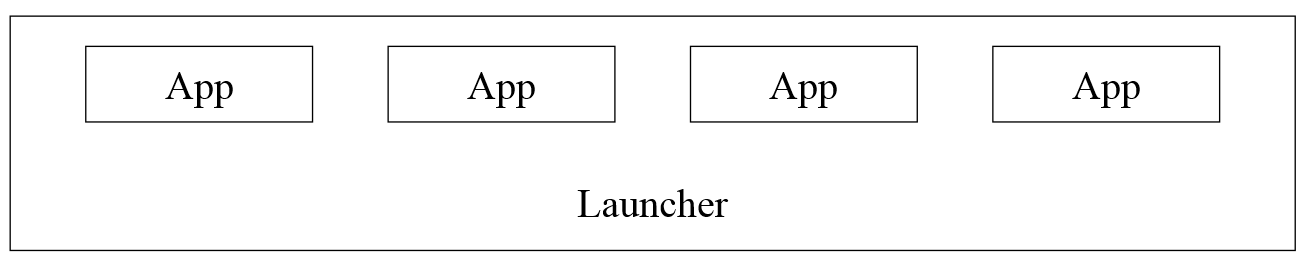
\includegraphics[width= 0.8 \textwidth]{pictures/NewLauncher.png}
		\end{figure}
	\end{center}
\end{frame}				% package solution + the rest by Sean
\section{Conclusion}
\subsection{Conclusion}
\begin{frame}
	\frametitle{Conclusion}
\end{frame}

\begin{frame}
	\frametitle{The overall project}
	\begin{figure}[H]
		\centering
		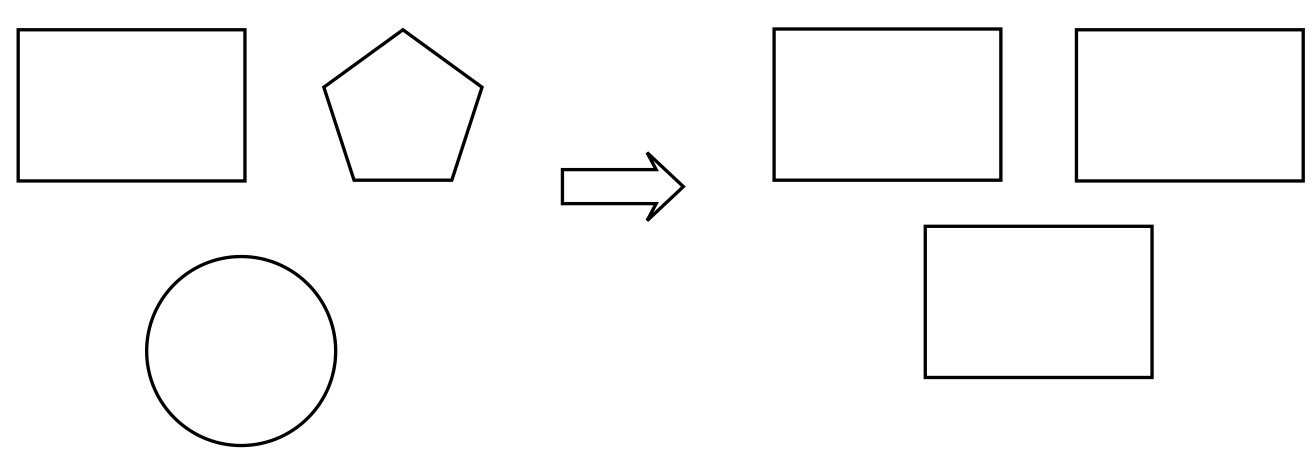
\includegraphics[width= 0.8 \textwidth]{pictures/SameGUIDesign.png}
	\end{figure}
\end{frame}

\begin{frame}
	\frametitle{Google play and analytics}
	\begin{itemize}
		\item Supervised
		\item Version control
		\item Name change
	\end{itemize}
\end{frame}

\begin{frame}
	\frametitle{Build structure}
	\begin{figure}[H]
		\centering
		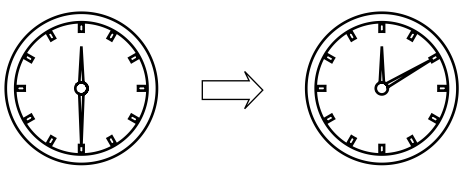
\includegraphics[width= 0.8 \textwidth]{pictures/Buildtime.png}
	\end{figure}
\end{frame}

\begin{frame}
	\frametitle{Product owner}
	\begin{itemize}
		\item Improved work flow for B\&D
		\item Shared user stories
		\item Combined backlog
	\end{itemize}
\end{frame}

\section{Recommendation and reflexion}
\subsection{Recommendation and reflexion}
\begin{frame}
	\frametitle{Recommendation and reflexion}
\end{frame}

\begin{frame}
	\frametitle{Product owner}
	\begin{itemize}
		\item Important role
		\item One per subproject
	\end{itemize}
\end{frame}

\begin{frame}
	\frametitle{User stories}
	\begin{itemize}
		\item Standardization is good
		\item Improve the existing
	\end{itemize}
\end{frame}

\begin{frame}
	\frametitle{Redmine}
	\begin{itemize}
		\item Good for wiki pages
		\item Not good for user stories
		\item A new tool for user stories should be found
	\end{itemize}
\end{frame}

\begin{frame}
	\frametitle{Rename}
	\begin{itemize}
		\item Rename needed for "Ugeplan"
		\item A lot of work
		\item Only rename if absolutely necessary
		\item Renaming effect a lot of groups
	\end{itemize}
\end{frame}

\begin{frame}
	\frametitle{Package}
	\begin{itemize}
		\item If Google make collections
			\begin{itemize}
				\item Make a collection for all the apps
			\end{itemize}
		\item Else
			\begin{itemize}
				\item Combine all the apps in the launcher
				\item Do it as early as possible
			\end{itemize}
	\end{itemize}
\end{frame}

\begin{frame}
	\frametitle{Backup}
	\begin{itemize}
		\item Server has backup
		\item Saves backup internally
		\item Backup should be saved externally
	\end{itemize}
\end{frame}

\begin{frame}
	\frametitle{Leadership}
	\begin{itemize}
		\item A good leader is important
		\item Improve the work flow
		\item Improve collaboration in the project
	\end{itemize}
\end{frame}

\begin{frame}
	\frametitle{Subprojects}
	\begin{itemize}
		\item Good to use
		\item Usefull for dividing responsibilities
		\item More focus on GUI
	\end{itemize}
\end{frame}

\begin{frame}
	\frametitle{Scrum}
	\begin{itemize}
		\item Good for multiprojects
		\item Recommend that groups use it
	\end{itemize}
\end{frame}

\begin{frame}
	\frametitle{Work time and place}
	\begin{itemize}
		\item Worked at the university
		\item Better contact with other groups
		\item Better work flow
	\end{itemize}
\end{frame}
				%Conclusion and reflection by Sean

% Make an empty last page
\begin{frame}
\end{frame}

\end{document}